%Please use LuaLaTeX or XeLaTeX
\documentclass[11pt,aspectratio=169]{beamer}

\usepackage[ngerman]{babel}
\usepackage{ragged2e}

\definecolor{ethblue}{RGB}{32, 91, 174}
\definecolor{mygrey}{RGB}{175, 175, 175}

\hypersetup{
  colorlinks=true,
  urlcolor=ethblue,
  linkcolor=ethblue,
  citecolor=ethblue
}

\title{Theoretische Informatik}
% \date[ABC 2021]{24. Sep 2026}
\date[]{1. Okt 2026}
\author{Olivér Kovács}
% \institute{Organizational Unit\\can spread over 2 lines}

\usetheme{eth}

\colorlet{titlefgcolor}{ETHBlue}
\colorlet{accentcolor}{ETHRed}

\begin{document}

%\def\titlefigure{elements/title-page-image}		% Default image
%\def\titlefigure{elements/title-page-image-43}	% Use this for 4:3 presentations

\titleframe

% \tocframe

% \section{Layout}

\begin{frame}{Hallo!}
    \begin{columns}
        \begin{column}{0.6\textwidth}
            Meine Webseite: \href{https://oliverkovacs.dev/ti}{oliverkovacs.dev/ti}

            \vspace{2em}

            Ich bin jederzeit erreichbar: \\
            \href{tel:REDACTED}{REDACTED (WA)} \\
            \href{mailto:okovacs@ethz.ch}{okovacs@ethz.ch}
        \end{column}
        \begin{column}{0.3\textwidth}
            
\includegraphics[width=0.8\columnwidth]{img/qr}
        \end{column}
    \end{columns}
\end{frame}

\begin{frame}{Übersicht}
    \begin{enumerate}
        \item Formalisierung
        \item Formalismus einsetzen (Wir sind hier!)
        \item \textcolor{mygrey}{Berechenbarkeit}
        \item \textcolor{mygrey}{Komplexitätstheorie}
    \end{enumerate}
\end{frame}

\begin{frame}{Serien}
    In Gruppen abgeben!

    \vspace{1em}

    Mehr begründen!

    \vspace{1em}

    Das leere Wort (\(\lambda\))
\end{frame}

\begin{frame}{Quiz Frage 1}
    \begin{center}
        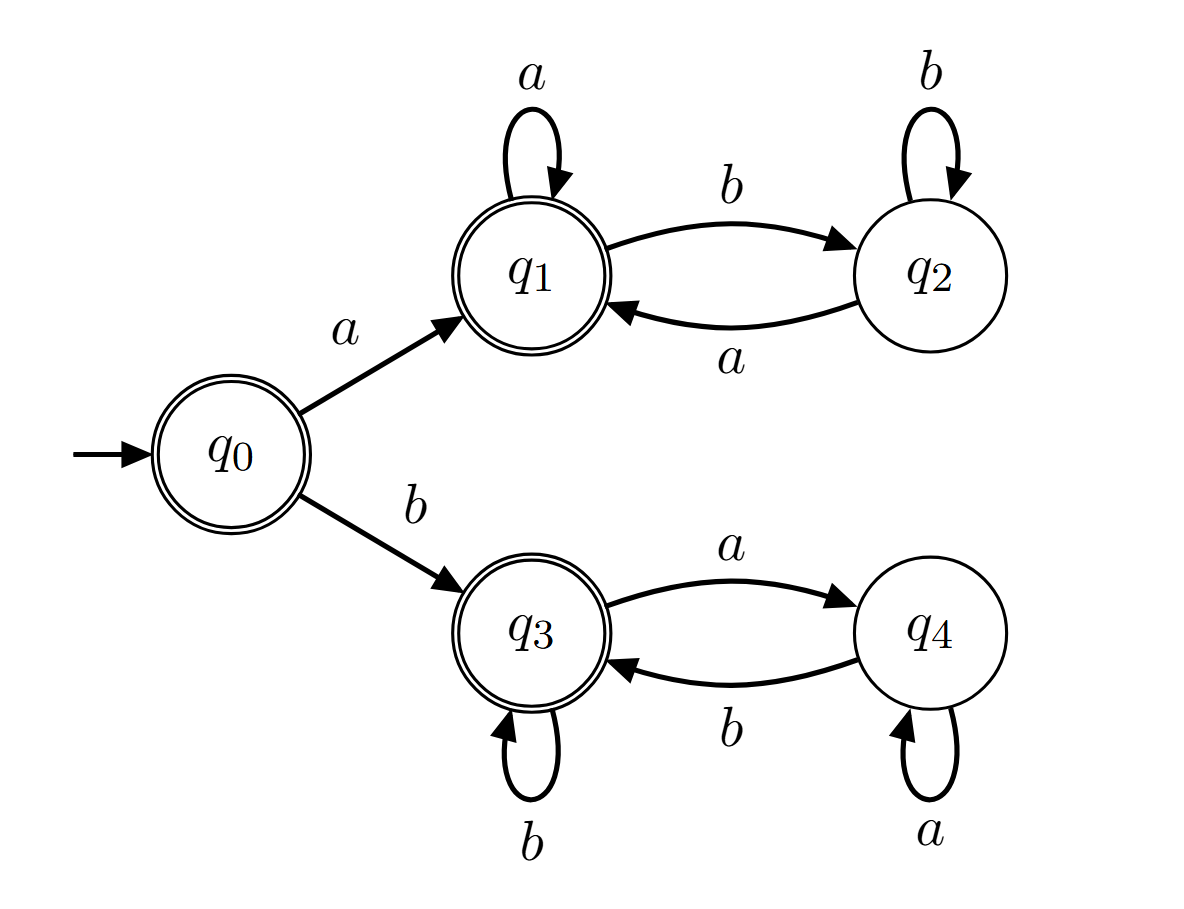
\includegraphics[width=10em]{img/f1}
    \end{center}
    \begin{enumerate}
        \item \(L_1 = \{ w \in \{ a, b \}^* \mid w \text{ enthät das Teilwort } ab \text{ gleich oft wie } ba \}\)
        \item \(L_2 = \{ w \in \{ a, b \}^* \mid w = xv, x \in \{ a, b \}, 2|v|_x \ge |v| \}\)
        \item \(L_3 = \{ w \in \{ a, b \}^* \mid w = \lambda \lor (w = w_1 \ldots w_{|w|} \land w_1 = w_{|w|})\}\)
        \item \(L_4 = \{ w \in \{ a, b \}^* \mid w \text{ endet nicht in } ab \text{ oder } ba \}\)
    \end{enumerate}
\end{frame}

\begin{frame}{Quiz Frage 2}
    \begin{center}
        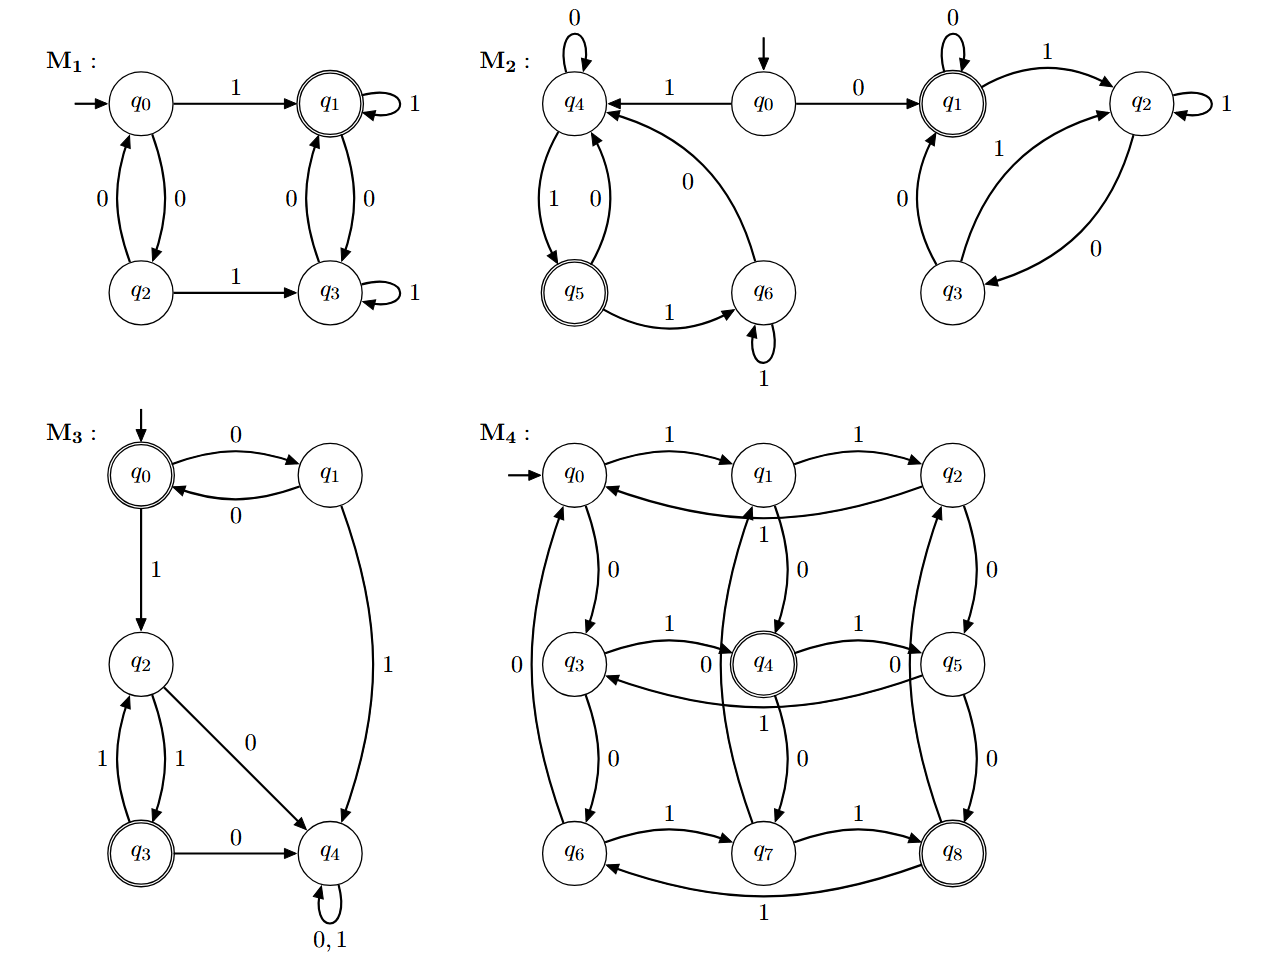
\includegraphics[width=20em]{img/f2}
    \end{center}
\end{frame}

\begin{frame}{Quiz Frage 2}
    \begin{center}
        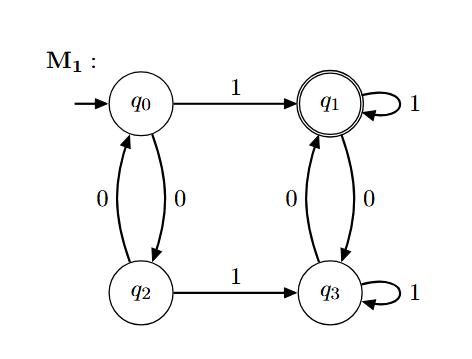
\includegraphics[width=12em]{img/f21}
    \end{center}
    \begin{enumerate}
        \item \(L = \{ w \in \{ 0, 1 \}^* \mid |w|_0 \cdot |w|_1 \equiv 1 \mod 3 \}\)
        \item \(L = \{0^{2k} 1^{2l} \mid k, k \in \mathbb N\}\)
        \item \(L = \{ w \in \{ 0, 1 \}^* \mid (|w|_0)^{|w|_1} \equiv 0 \mod 2\}\)
        \item \(L = \{ xw \in \{ 0, 1 \}^* \mid x \in \{ 0, 1 \} \text{ und Nummer}(w) \equiv x  \mod 4\}\)
    \end{enumerate}
\end{frame}

\begin{frame}{Quiz Frage 2}
    \begin{center}
        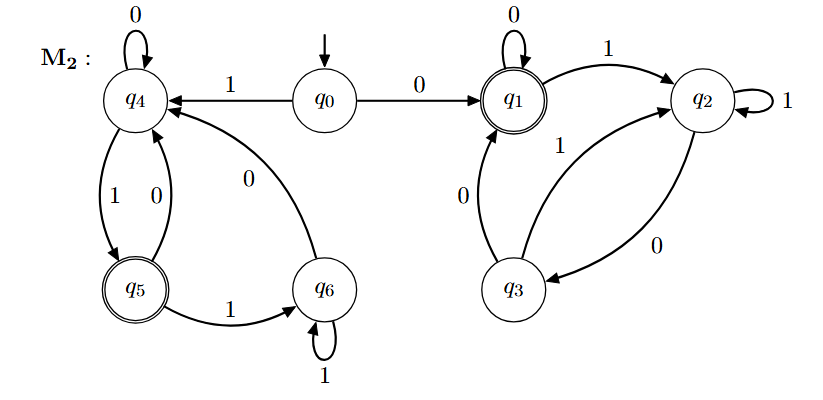
\includegraphics[width=15em]{img/f22}
    \end{center}
    \begin{enumerate}
        \item \(L = \{ w \in \{ 0, 1 \}^* \mid |w|_0 \cdot |w|_1 \equiv 1 \mod 3 \}\)
        \item \(L = \{0^{2k} 1^{2l} \mid k, l \in \mathbb N\}\)
        \item \(L = \{ w \in \{ 0, 1 \}^* \mid (|w|_0)^{|w|_1} \equiv 0 \mod 2\}\)
        \item \(L = \{ xw \in \{ 0, 1 \}^* \mid x \in \{ 0, 1 \} \text{ und Nummer}(w) \equiv x  \mod 4\}\)
    \end{enumerate}
\end{frame}

\begin{frame}{Quiz Frage 2}
    \begin{columns}
        \begin{column}{0.2\textwidth}
            \begin{center}
                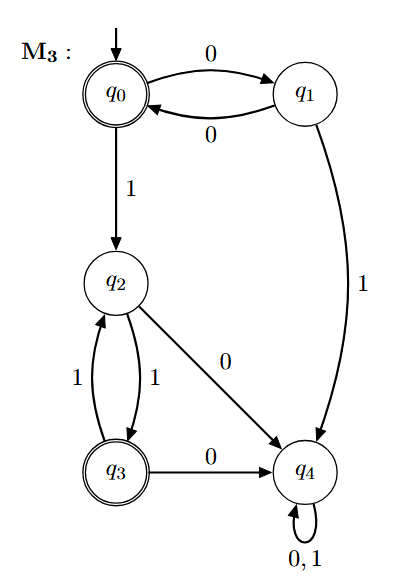
\includegraphics[width=10em]{img/f23}
            \end{center}
        \end{column}
        \begin{column}{0.6\textwidth}
            \begin{enumerate}
                \item \(L = \{ w \in \{ 0, 1 \}^* \mid |w|_0 \cdot |w|_1 \equiv 1 \mod 3 \}\)
                \item \(L = \{0^{2k} 1^{2l} \mid k, l \in \mathbb N\}\)
                \item \(L = \{ w \in \{ 0, 1 \}^* \mid (|w|_0)^{|w|_1} \equiv 0 \mod 2\}\)
            \item \(L = \{ xw \in \{ 0, 1 \}^* \mid x \in \{ 0, 1 \} \text{ und }\) \\
            \( \text{Nummer}(w) \equiv x  \mod 4\}\)
            \end{enumerate}
        \end{column}
    \end{columns}
\end{frame}

\begin{frame}{Quiz Frage 2}
    \begin{columns}
        \begin{column}{0.2\textwidth}
            \begin{center}
                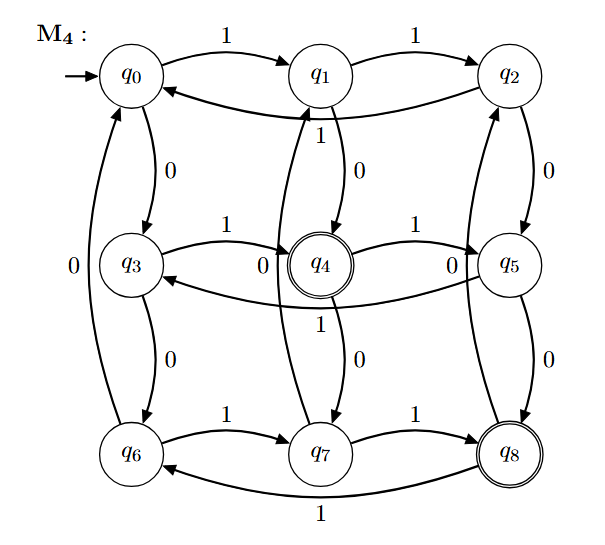
\includegraphics[width=11em]{img/f24}
            \end{center}
        \end{column}
        \begin{column}{0.6\textwidth}
            \begin{enumerate}
                \item \(L = \{ w \in \{ 0, 1 \}^* \mid |w|_0 \cdot |w|_1 \equiv 1 \mod 3 \}\)
                \item \(L = \{0^{2k} 1^{2l} \mid k, l \in \mathbb N\}\)
                \item \(L = \{ w \in \{ 0, 1 \}^* \mid (|w|_0)^{|w|_1} \equiv 0 \mod 2\}\)
            \item \(L = \{ xw \in \{ 0, 1 \}^* \mid x \in \{ 0, 1 \} \text{ und }\) \\
            \( \text{Nummer}(w) \equiv x  \mod 4\}\)
            \end{enumerate}
        \end{column}
    \end{columns}
\end{frame}

\begin{frame}{Quiz Frage 3}
    \begin{center}
        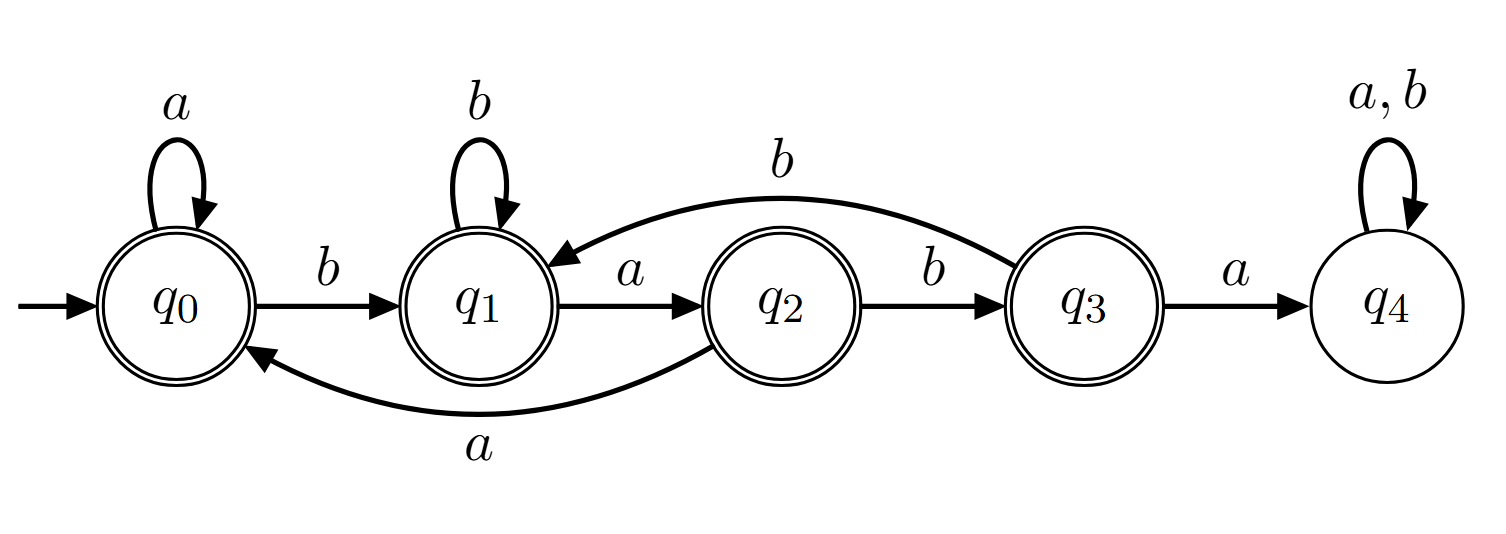
\includegraphics[width=20em]{img/f3}
    \end{center}

    Erkennt die Sprache \(L = \{ w \in \{a, b\}* \mid w \text{ enthält } baba \text{ nicht als Teilwort } \}\).

    \vspace{1em}

    Ändere die ausgehenden Übergänge eines Zustands so, dass
    der Automat stattdessen \(L' = \{ w \in \{ a, b \}^* \mid w \text{ endet nicht auf } baba \}\) erkennt.
\end{frame}


\begin{frame}{Regularität}
    \textbf{Definition 3.1.}
    [...] \(\mathcal L_{\text{EA}} = \{ L(M) \mid M \text{ ist EA }\}\) ist die \textit{Klasse der regulären Sprachen}.
    Jede Sprache \(L \in \mathcal L_{\text{EA}}\) wird \textit{regulär} genannt.
\end{frame}

\begin{frame}{Wie zeigt man Nichtregularität?}
    \textbf{Lemma 3.3.}
    Sei \(A = (Q, \Sigma, \delta_A, q_0, F)\) ein EA.
    Seien \(x, y \in \Sigma^*, x \neq y\), so dass
    \[
        (q_0, x) \vdash_A^* (p, \lambda) \text{ und }
        (q_0, y) \vdash_A^* (p, \lambda)
    \]
    für ein \(p \in Q\) gilt.
    Dann existiert für jedes \(z \in \Sigma^*\) ein \(r \in Q\),
    so dass \(xz, yz \in \text{Kl}[r]\).
    Insbesondere gilt
    \[
        xz \in L(A) \iff yz \in L(A).   
    \]
\end{frame}

\begin{frame}{Wie zeigt man Nichtregularität?}
    \justify
    \textbf{Korollar:}
    Sei \(A\) ein EA.
    Seien \(x, y\) zwei Wörter für die ein
    Suffix \(z\) existiert, so dass gilt
    \(xz \in L(A) \iff yz \not\in L(A)\), also
    \(|\{xz, yz\} \cap L(A)| = 1\).

    \vspace{0.5em}

    Dann müssen \(x\) und \(y\) in zwei verschiedenen Zustände landen.
\end{frame}

\begin{frame}{Wie zeigt man Nichtregularität?}
    \justify

    \textbf{Idee:} Nehme an, \(L\) sei regulär.
    Dann gibt es ein EA \(A\) mit \(L(A) = L\).
    Nehme an, \(A\) hat \(n\) Zustände. \\

    \vspace{0.5em}

    Finde \(n + 1\) solche Wörter \(x_0, \ldots, x_{n}\),
    dass für alle Paare \(x_i, x_j\) ein Suffix \(z_{i,j}\)
    existiert, so dass \(|\{x_i z_{i,j}, x_j z_{i,j}\} \cap L| = 1\).

    \vspace{0.5em}

    Dann müssen \(x_0, \ldots, x_n\) in paarweise verschiedene Zustände landen. Das ist ein Wiederspruch.
\end{frame}

\begin{frame}{Nebenbemerkung}
    \begin{center}
        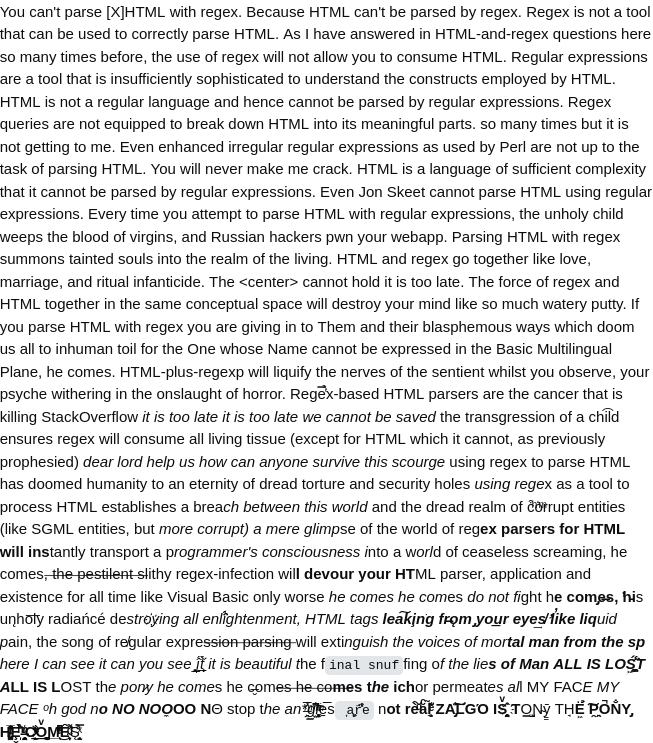
\includegraphics[width=14em]{img/html}
    \end{center}
\end{frame}

\begin{frame}{Nebenbemerkung}
    \textit{"HTML is not a regular language and hence cannot be parsed by regular expressions."}
    (\href{https://stackoverflow.com/questions/1732348/regex-match-open-tags-except-xhtml-self-contained-tags}{https://stackoverflow.com/questions/1732348/regex-match-open-tags-except-xhtml-self-contained-tags})

    \vspace{2em}

    Aber warum?
\end{frame}

% \setbeamertemplate{footline}{}

\begin{frame}{Aufgaben}

    \begin{enumerate}
        \justifying
        \item \textbf{Aufgabe 1.}
            Sei \(L_1 = \{w \in \{ a, b \}^* \mid |w| \ge 3 \text{ oder } |w|_a = |w|_b\}\).
            Konstruiere einen EA \(A\) mit \(L(A) = L_1\).

        \item \textbf{Aufgabe 2.}
            Sei \(L_2 = \{a^nb^m \mid n, m \in \mathbb N, 2 \le m \le n - 1, m \text{ ist Teiler von } n\}\).
            Beweise unter Zuhilfenahme von Lemma 3.3., dass \(L_2\) nicht regulär ist.

        \item \textbf{Aufgabe 3.}
            Ein EA \(A\) heisst minimal, falls kein kleinerer EA \(B\)
            mit \(L(A) = L(B)\) existiert.
            Konstruiere einen minimalen EA \(A\) mit \(L(A) = L_1\).
            Beweise unter Zuhilfenahme von Lemma 3.3., dass \(A\) minimal ist.

        \item \textbf{Aufgabe (Bonus)}
            Beweise, dass HTML keine reguläre Sprache ist. :) \\
            \vspace{0.5em}
            \textit{Hint: Du kannst äquivalenterweise beweisen, dass die Sprache} \(L_{\text{Klammer}} = \{ w \in \{ \boxed(, \boxed) \}^* \mid w \text{ ist eine valide Verschachtelung von Klammern}\}\) \textit{nicht}

            \textit{regulär ist.}
    \end{enumerate}
\end{frame}

\end{document}.
